\documentclass[12pt,a4paper]{article}
\usepackage[utf8]{inputenc}
\usepackage{amsmath}
\usepackage{amsfonts}
\usepackage{amssymb}
\usepackage{supertabular}
\usepackage{tabularx}
\usepackage{graphicx}
\usepackage{pdfpages}
\parskip=0pt
\usepackage[left=1in,right=1in,top=1in,bottom=1in]{geometry}
\title{\center{\textbf{\Large{System and Software Design Description(SSDD):}\\
\large{Incorporating Architectural Views and Detailed Design Criteria}\\
\normalsize{For}\\
\large{Swords and Sorcery}}}\\}
\author{Keith Drew,...}
\begin{document}
\maketitle
\pagebreak
\setcounter{tocdepth}{3}
\renewcommand\contentsname{\center{Swords and Sorcery Design\\Table of Contents}}
\tableofcontents

\section{Introduction}
This is the System and Software Design Document for Swords and Sorcery. This is one of five documents that describe the computer adaptation of the Swords and Sorcery board game developed by the Software Engineering class at the University of Idaho in Spring 2014.
\subsection{Document Purpose, Context, and Intended Audience}
\subsubsection{Document Purpose}
The purpose of this document is to describe the system and software design of Swords and Sorcery. 
\subsubsection{Document Context}
This document is written as part of a larger document that describes the Swords and Sorcery project developed by the CS383 students at University of Idaho, in Spring 2014. This document only describes the system and software design of the project, which is only a subset of the project.
\subsubsection{Intended Audience}
This document is intended to be read by Dr. Clinton Jeffery and members of the class, as well as any interested members of the University of Idaho Computer Science department. This document is not intended to be distributed publicly in any way.
\subsection{Software Purpose, Context, and Intended Audience}
\subsubsection{System and Software Purpose}
The purpose of the Swords and Sorcery system and software is to provide a computer adaptation of the complex board game of the same name. The system is designed to provide multiplayer functionality over the internet, and to simplify the complex rules of the original Swords and Sorcery.
\subsubsection{System and Software Context}
The context of this project is, again, restrained to the classroom, as it is an educational project, not intended for distribution. However, the source code for the project, as well as many resources, are available publicly on github.com. 
\subsubsection{Intended Users of System and Software}
The intended users of the Swords and Sorcery system are...
\subsection{Definitions, Acronyms, and Abbreviations}
\begin{center}
\begin{tabularx}{\linewidth}{|p{1.5in}|X|}\hline
\textbf{Term} & \textbf{Definition}\\
\hline
AD & Architectural Description: \"A collection of products to document an architecture.\"\space ISO/IEC 42010:2007\\
\hline
Alpha Test & Limited release(s) to selected, outside testers.\\
\hline
Architectural View & \"A representation of a whole system from the perspective of a related set of concerns.\"\space ISO/IEC 42010:2007\\
\hline
Architecture & \"The fundamental organization of a system embodied in its components, their relationships to each other, and to the environment, and the principles guiding its design and evolution.\"\space ISO/IEC 42010:2007\\
\hline
Beta Test & Limited release(s) to cooperating customers wanting early access to developing systems.\\
\hline
Client & The process the user directly interacts with, containing, among other things, the GUI.\\
\hline
Design Entity & \"An element (component) of a design that is structurally and functionally distinct from other elements and that is separately named and referenced.\"\space IEEE STD 1016-1998\\
\hline
Design View & \"A subset of design entity attribute information that is specifically suited to the needs of a software project activity.\"\space IEEE STD 1016-1998\\
\hline
Edge & The edge between two hexes. Edges can include roads, walls, streams, etc. and can effect movement or combat\\
\hline
GUI & Graphical User Interface - What the user sees and interacts with - also called the HUD.\\
\hline
Hexagon & A hexagon shaped location on the game or diplomacy map that can contain things like units, edges, or terrain. Or the mathematical hexagon shape.\\
\hline
HUD & Heads Up Display - What the user sees, with respect to interface - also called the GUI.\\
\hline
IP & Internet Protocol - Typically refers to an IP Address.\\
\hline
S\&S & Swords and Sorcery\\
\hline
Server & The (single) process that a client connects and sends messages to. \\
\hline
SSDD & System and Software Design Document\\
\hline
SSRS & System and Software Requirements Specification\\
\hline
System & \"A collection of components organized to accomplish a specific function or set of functions.\"\space ISO/IEC 42010:2007\\
\hline
System Stakeholder & \"An individual, team, or organization (or classes thereof) with interests in, or concerns, relative to, a system.\"\space ISO/IEC 42010:2007\\
\hline
\end{tabularx}
\end{center}

\subsection{Document References}
\begin{enumerate}
\item CSDS, textit{System and Software Requirements Specification Template}, Version 1.0, July
31, 2008, Center for Secure and Dependable Systems, University of Idaho, Moscow, ID, 83844.

\item ISO/IEC/IEEE, \textit{IEEE Std 1471-2000 Systems and software engineering -- Recommended practice for architectural description of software intensive systems,} First edition 2007-07-15, International Organization for Standardization and International Electrotechnical Commission, (ISO/IEC), Case postale 56, CH-1211 Geneve 20, Switzerland, and The Institute of Electrical and Electronics Engineers, Inc., (IEEE), 445 Hoes Lane, Piscataway, NJ 08854, USA.

\item IEEE, \textit{IEEE Std 1016-1998 Recommended Practice for Software Design Descriptions}, 1998-09-23, The Institute of Electrical and Electronics Engineers, Inc., (IEEE) 445 Hoes Lane, Piscataway, NJ 08854, USA.

\item 3) ISO/IEC/IEEE, \textit{IEEE Std. 15288-2008 Systems and Software Engineering -- System life cycle processes,}Second edition 2008-02-01, International Organization for Standardization and International Electrotechnical Commission, (ISO/IEC), Case postale 56, CH-1211 Geneve 20, Switzerland, and The Institute of Electrical and Electronics Engineers, Inc., (IEEE), 445 Hoes Lane, Piscataway, NJ 08854, USA.

\item ISO/IEC/IEEE, IEEE Std. 12207-2008, \textit{Systems and software engineering -- Software life cycle processes}, Second edition 2008-02-01, International Organization for Standardization and International Electrotechnical Commission, (ISO/IEC), Case postale 56, CH-1211 Geneve 20, Switzerland, and The Institute of Electrical and Electronics Engineers, Inc., (IEEE), 445 Hoes Lane, Piscataway, NJ 08854, USA.
\end{enumerate}

\subsection{Overview of Document}
\paragraph{Section 2} of this document describes the concerns and constraints of the system and software, with respect to environmental constraints, system requirement constraints, and user characteristic constraints. Section 2 also describes stakeholder concerns.
\paragraph{Section 3} of this document describes the System and Software architecture of Swords and Sorcery, from different points of view, namely the user's point of view and the developer's point of view.
\paragraph{Section 4} of this document describes the finer details of the software design, listing software and system components that are crucial to the operation of the Swords and Sorcery game. 
\paragraph{Section 5} of this document describes the requirements traceability of the Swords and Sorcery project, highlighting how our original project requirements have been met, modified, and implemented.
\subsection{Document Restrictions}
This document is for LIMITED USE ONLY to UI CS personnel working on the project.
\section{Constraints and Concerns}

\subsection{Constraints}
Swords and Sorcery requires the Java Runtime Environment 8 to run. S\&S also requires the JDK 8.0 and Netbeans 8.0 or better to develop. The game will run on Windows, Mac, and Linux, provided those systems have the mentioned software packages (JRE to play, JDK/Netbeans to develop). To play the game, a network connection is required, as well as the IP Address of the game server. As S\&S is a multiplayer game, one client is required for each player. Typically, this should be done using multiple computers, however, multiple clients can be run on the same computer.

\subsection{Stakeholder Concerns}
There are no financial stakeholders, however, Dr. Clinton Jeffery can be considered a stakeholder, as well as each class member. As a class member, our concerns are providing a quality product, while Dr. Jeffery's concerns may include using good design principles, as this is a Software Engineering course. 
Other concerns include design requirements such as portability, 

\section{System and Software Architecture}
\subsection{Developer's Architectural View}
\subsubsection{Developer's View Identification}
There are multiple developer views within the scope of the S\&S project for CS383. The views represent each subteam, and there are three subteams - HUD Team, Rules Team, and Networking Team. The descriptions of each sub-view follow, as well as an overview diagram.
\paragraph{Architectural Overview}
The following class diagram is inaccurate with respect to the project as it currently stands. The inaccuracies are the Chart class, which does not exist, and we discovered is unnecessary, as well as the alliance and player classes, which were never created. The alliance class was never created because we didn't make it that far with the project, and the player class was replaced with flags and variables, as a class was determined to be unneeded. 
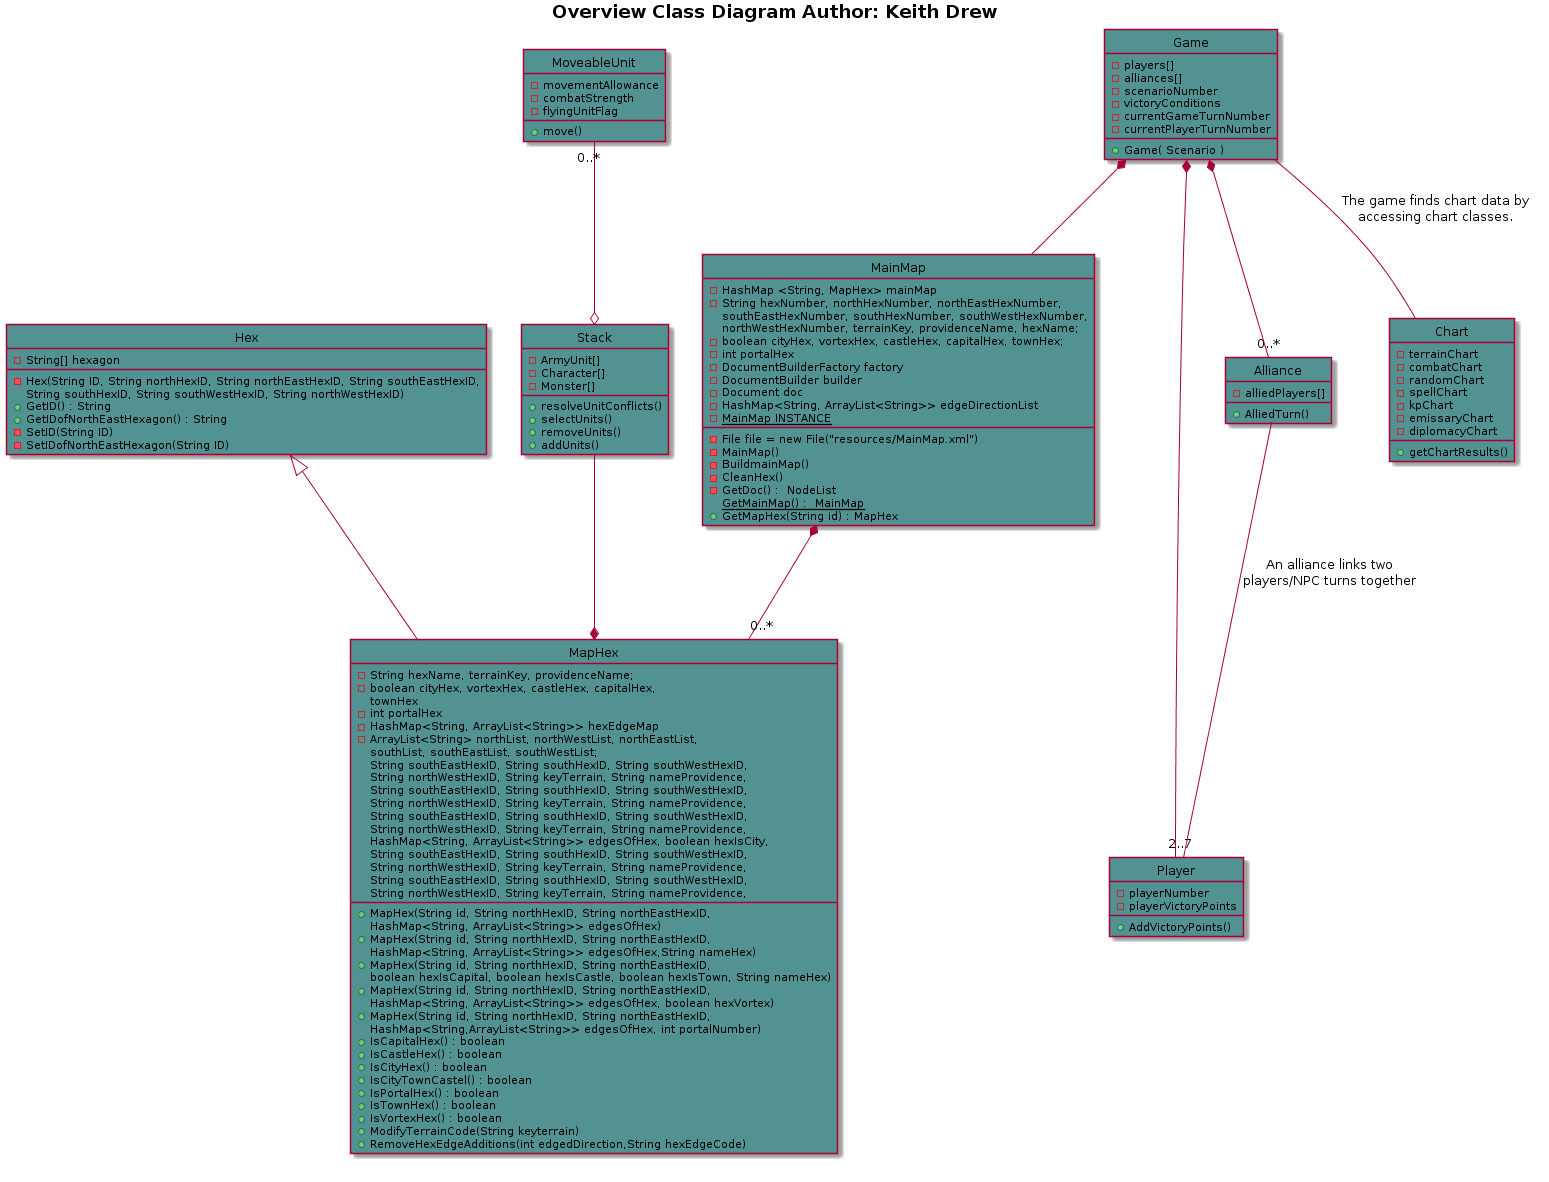
\includepdf{overview.png}
\paragraph{HUD Team View} The HUD Team view includes all software design related to the HUD/GUI and handles how the user(s) interact with the S\&S game rules and networking. 
\paragraph{Rules Team View} The Rules Team view includes all software implementations of the S\&S rule set, some of which overlaps with other views. Typically, Rules Team is in charge of implementing internal logic and data structures.
\paragraph{Networking Team View} The Networking Team view includes all network communication related to the S\&S game. This includes the client/server model, the communication protocols, the server setup and more.
\subsubsection{Developer's View Representation and Description}
\paragraph{HUD Team View Representation and Description}
[Insert Description of graphics (UML) here] 
%\includegraphics[scale=•]{•}
\paragraph{Rules Team View Representation and Description}
[Insert Description of graphics (UML) here]
%\includegraphics[scale=•]{•}
\paragraph{Networking Team View Representation and Description}
[Insert Description of graphics (UML) here]
%\includegraphics[scale=•]{•}
\subsubsection{Developer's Architectural Rationale} it breaks without text so often it seems

\subsection{User's Architectural View}
	\subsubsection{User's View Identification}
	\subsubsection{User's View Representation and Description}
\subsection{Consistency of Architectural Views}
	\subsubsection{Detail of Inconsistencies Between Architectural Views}
	\subsubsection{Consistency Analysis and Inconsistency Mitigations}

\section{Software Detailed Design}
	\subsection{Developer's Viewpoint Detailed Software Design}

\pagebreak
\subsection{Component Dictionary}
\small{
\begin{center}
\noindent\begin{tabularx}{\linewidth}{|l|X|X|X|X|}\hline
\textbf{Name} & \textbf{Type/Range} & \textbf{Purpose} & \textbf{Dependencies} & \textbf{Subordinates}\\
\hline
Army Combat Result Table & Static Method & Determine results of combat lookup & Two ArrayLists: Attackers, Defenders & None\\
\hline
Army Unit & Class & Unit SubClass & Moveable Unit & All individual unit types\\
\hline
Characters & Class & Unit SubClass & Moveable Unit & None\\
\hline
ClientObject & Class & Represents an open connection to a client from the server. & Tag, Flag, MessagePhoenix \\
\hline
Conductor & Class & Contains public handler methods for incoming network methods. & Tag, Flag & \\
\hline
Flag & Enum Class & An enumerate constant class providing identifiers for each concrete type of network message. & & \\
\hline
Hexagon Classes & Model & Represents a hexagon & Hex Edge Classes, Terrain Classes, UnitPool & \\
\hline
Hex Edge Classes & Model & Classes to collect and represent elements on hexagon edges & Hex Classes & \\
\hline
Hexagon Map Classes & Model & Classes to represent a "map" of hexagons, either diplomacy or game. & Hex Classes & \\
\hline
Lobby & Class & A server-side object that manages a grouping of client connection. & Tag, Flag, MessagePhoenix & \\ 
\hline
MainMenuController & Controller & Define and limit access to main menu & Game.java & \\
\hline
Map Rendering Classes & View & Renders the game map and things on it & MapView, Hexagon Classes, Hex Edge Classes & \\
\hline
MapView & View & A GUI widget to act as a container for the Map Rendering code & Hexagon Classes, Map Rendering Classes & \\
\hline
MessagePhoenix & Utility Class & Used to pack, unpack, send and receive messages over the network & Tag, Flag & \\
\hline
Moveable Unit & Class & Unit SuperClass & None & ArmyUnit, Character, Monster\\
\hline
MovementCalculator & Static Class & Determine Legal Moves & UnitPool, MainMap & Retreat/Move\\
\hline
NetworkClient & Class & Manages network connection for client. & Tag, Flag, MessagePhoenix & Conductor \\
\hline
NetworkServer & Class and Process & The independent server process that clients connect to. & Tag, Flag, MessagePhoenix & ClientObject\\
\hline
Tag & Enum Class & An enumerated constant class providing identifiers for each general type of network message. & & \\
\hline
\end{tabularx}
\end{center}
}

\subsection{Component Detailed Design}
\subsection{Detailed Design for Component: Army Unit}
\paragraph{Purpose} This class contains the data of the Army Units in the game and extends the Movable Unit class. This class contains new data like the strength of a unit and whether or not the units is conjured or demoralized. If a unit is conjured then there are special member variables that contain values that are associated with conjured units. If a unit is demoralized then the strength of the unit is different so a demoralized strength variable was added to the class. The strength and demoralized strength variables are used during the combat phase of a users turn and is used to determine the outcome of combat. 
\paragraph{Input} The only Inputs to this class are the ones needed to fill the member variables of this class.
\paragraph{Output} This class by itself has no output produced other than the getter functions in the class.
\paragraph{Process} Output is obtained by calling the getter functions. 
\paragraph{Design Constraints and Performance Requirements}	In order for this class to preform correctly all of the needed variables need to be filled out.

\subsection{Detailed Design for Component: Army Combat Results Table}
\paragraph{Purpose} The purpose of this method is a lookup for the results of Combat. 
\paragraph{Input} Input needs to be two Array Lists: one is called attackers and one defenders. Also the hex object that the defenders are positioned on is needed. The attackers array list is comprised of all of the attacking Army Units in the combat and the defenders are all of the defending Army Units in the combat. The defenders hex is needed in order to calculate the defence multipliers that the defending units get from the terrain values of the hex object.
\paragraph{Output} The output of this function is a simple 2 value array corresponding the result of the combat. The first value is what's required of the attackers and the second value is what's required of the defenders. A -1 means the units were killed, a 0 means that there was no result of the combat and any positive number represents the number of hexes a unit has to retreat. 
\paragraph{Process} The function adds the total strengths of both the attackers and defenders. Then applies the terrain multiplier to the defenders total strength. Finally the ratio of attackers over defenders plus a random dice roll determines the outcome of the combat.  
\paragraph{Design Constraints and Performance Requirements} One design constraint of the table was that in the game the ratio's have to be reduced to the smallest possible fraction in favour of the defending units. To work around this and index was made to match the determined ratio to the correct look up value on the table. Also the units strength and race is required to be filled out in order for this function to work properly. 

\subsection{Detailed Design for Component: Conductor}
\paragraph{Purpose} The Conductor class is used by the client. When NetworkClient detects an incoming message that alters the state of the game (such as a unit being moved), it calls a method inside of the Conductor class. The purpose of putting handler code in the Conductor class rather than inside of NetworkClient was to seperate the code in NetworkClient that deal with internal networking objects (like sockets) from the code that deals with other game object (like unitPool).
\paragraph{Input} Each message in the Conductor class is invoked with parameters received via an incoming network message.
\paragraph{Output} The methods in the Conductor class may respond to an incoming message through any public interface. For example, the Conductor class may alter UnitPool in response to a network message.
\paragraph{Process} An incoming message is received inside of NetworkClient. NetworkClient determines the type of message, and forwards the message to Conductor is appropriate. Conductor checks the tag of the message, to determine the message type, and calls the appropriate code for the message type.
\paragraph{Design Constraints and Performance Requirements} Conductor was designed to let other team members work conveniently with networking code, without having to stare at networking internal details.


\subsection{Detailed Design for Component: MessagePhoenix}
\paragraph{Purpose} MessagePhoenix contains the methods to create, send, and receive messages over the network. This functionality is used by both the client and server. MessagePhoenix is intended to be called indirectly by client code through NetworkClient, (as well as by the Server).
\paragraph{Input} MessagePhoenix requires a reference to an input or output object stream associated with a network socket. The utility methods in MessagePhoenix also accept any number of Objects (using a variable length parameter list), which will be packaged and sent over the network. The first two objects of a message must be a Flag and Tag, which identify the message. 
\paragraph{Output} MessagePhoenix can return the NetworkPacket received from a network connection. 
\paragraph{Process} Receiving a message initiates a blocking read from the network socket. Sending a message writes to the network socket immediately. 
\paragraph{Design Constraints and Performance Requirements} MessagePhoenix needs to accomodate a variety of message types. 

\subsection{Detailed Design for Component: ClientObject }
\paragraph{Purpose} ClientObject is used by the server. ClientObject is a class which represents a client who has connected to the server. ClientObject is not something that runs on the client machine. NetworkServer creates an instance of ClientObject for each new connection to the server. ClientObject is responsible for the socket to the client. The main activity of a ClientObject instance is to listen for incoming messages from the client represented by the ClientObject, which it accomplishes by an independent thread, and to send messages to the client through the network socket.
\paragraph{Input} ClientObject receives messages from the associated client. 
\paragraph{Output} NetworkServer and other ClientObjects are allowed
to send message to the associated client through ClientObject.
\paragraph{Process} ClientObject's listener thread reads and process messages from the connected client. Other threads request the writer
\paragraph{Design Constraints and Performance Requirements}

\subsection{Detailed Design for Component: NetworkClient }
\paragraph{Purpose} NetworkClient is used by the client. NetworkClient provides an interface that other client-side components can use to interact with the network. NetworkClient creates the connection to the server, and sends and receives messages over the network.
\paragraph{Input} NetworkClient listens for incoming messages from the network. Some messages impact the internal state of NetworkClient, and other messages are forwarded to Conductor.
\paragraph{Output} NetworkClient provides a public interface for sending message over the network.
\paragraph{Process} To send a message, NetworkClient uses MessagePhoenix along with the network socket. On receiving a message, NetworkClient may respond internally, or forward the message to Conductor is the message concerns non-networking parts of the code (like unit movement).
\paragraph{Design Constraints and Performance Requirements}
NetworkClient must be able to receive network message asynchronously. 

\subsection{Detailed Design for Component: NetworkServer }
\paragraph{Purpose} NetworkServer is the main process that runs on the server machine. It waits for incoming connection requests. It creates a ClientObject for each connected client, and manages the group of connected clients through their ClientObject representations. 
\paragraph{Input} NetworkServer receives connection requests from client processes.
\paragraph{Output} NetworkServer creates new threaded ClientObject instances for each connection.
\paragraph{Process} When a connection is opened, the ClientObject instances is created (initiating an exchange of information, like user names, between the client and server), and stored in a list of connections.
\paragraph{Design Constraints and Performance Requirements} NetworkServer must be efficient enough to handle the expected number of connections. For our puposes, the demands on the NetworkServer are fairly minimal, and few performance issues have arisen.

\subsection{Detailed Design for Component: Tag }
\paragraph{Purpose} The Tag class contains "message tags". A message tag is the second object in a network packet. The tag identifies the concrete type of message. For example, the ``SEND HANDLE'' tag identifies a message as containing the handle (the username) of the new connection. By examining the Tag of a message, we can correctly interpret the other contents of the message. 
\paragraph{Input} The Tag class receives no input. 
\paragraph{Output} The Tag class does not produce output. 
\paragraph{Process} None. 
\paragraph{Design Constraints and Performance Requirements} None.

\subsection{Detailed Design for Component: Flag }
\paragraph{Purpose} The Flag class contains "message flags". A message flag is the first object in a network packet. The flag identifies the general type of a message. For example, there is a "REQUEST" and "RESPONSE" flag. The motivation for this is because many interactions with the server follow a REQUEST, ACCEPT or DENY format. For example, you might ``REQUEST'' ``SEND HANDLE'' in one message, and expect a ``RESPONSE'' ``SEND HANDLE''.
\paragraph{Input} None.
\paragraph{Output} None.
\paragraph{Process} None.
\paragraph{Design Constraints and Performance Requirements} None.
	
\subsection{Detailed Design for Component: Lobby }
\paragraph{Purpose} The Lobby class is used by the server. Lobby represents a grouping of client connections (ClientObjects, which live on the server), and is used to manage a game instance. Lobby can remember things like the current turn. 
\paragraph{Input} A Lobby can receive messages from the NetworkServer, or forward messages from the connected ClientObjects. 
\paragraph{Output} A Lobby can forward messages received from one ClientObject to all clients in the Lobby.
\paragraph{Process} Clients are added to or removed from (by client request) a particular lobby. 
\paragraph{Design Constraints and Performance Requirements} None.

\subsection{Detailed Design for Component: Characters}
\paragraph{Purpose} This class contains the data of a Character in the game and extends the Movable Unit class. This class has variables unique to a character: magic level, magic potential, current manna, magic colour, and leadership. The magic level determines the hight level of spell that a character can cast. The magic potential is the maximum amount of manna that a character can have. The magic colour of a character determines when a character's spells have the most effect. Leadership is the influence that a character has in determining the result of army combat. Characters have the special ability to cast spells which uses the magic and manna values to determine the amount and effectiveness of their spells. 
\paragraph{Input} The only Inputs to this class are the ones needed to fill the member variables of this class.
\paragraph{Output} This class by itself has no output produced other than the getter functions in the class.
\paragraph{Process} Output is obtained by calling the getter functions. 
\paragraph{Design Constraints and Performance Requirements} In order for this class to preform correctly all of the member variables need to be filled out.
	
\subsection{Detailed Design for Component: Movable Unit}
\paragraph{Purpose} The purpose of this class is to have a common class of all moving units that the movement functions can access. This class is a super class of all units that can undergo a movement process. This allows for common data to be accessible by the appropriate functions. This common superclass also allows for the ability to store the data of all units in a single-typed data structure. This class contains member variables for movement allocation of a unit, the working movement allocation of a unit or the amount of movement left in a game turn, the race of the unit, the type of subclass that is inheriting from this class(such as armyUnit or Character), and the unique ID of the unit. The movement allocation of a unit is the amount of movement points allowed at the beginning of a turn then the working movement takes over. The working movement is used in order to keep track of how much a unit has move in a single turn. This allows for a user to partially move a unit in their turn then return to that unit and finish moving it later in the same turn. The race is used in many different calculations for units such as the movement cost per hex of a unit in a particular terrain. The subclass variable is used for typecasting the moveable unit back to the proper subclass in order for the subclass based operations to be executed. Finially the unique ID is used for network based communications to identify the unit that is being acted on. 
\paragraph{Input} Input needed to make this class function properly are values to fill the member variables of this class. 
\paragraph{Output} The only output of this class is by getters of the member variables of the class. 
\paragraph{Process} Call the getter functions.
\paragraph{Design Constraints and Performance Requirements} One constraint of this class was the necessity to be casted back into the appropriate subclass this was solved by creating the unitType(subclass Type) variable. Also in order for this class to preform right with other classes and functions all of the variables need to be set. 
	
\subsubsection{Detailed Design for Component: Movement Calculator}
\paragraph{Purpose} The movement calculator is a static java class that handles most forms of movement. 
\paragraph{Input} The movement calculator takes two inputs to generate a list of moves: the unit moving, and the hex object they are beginning from. To calculate a retreat, the movement calculator takes as input the unit retreating, the hex they are retreating from, and the number of hexes they are required to retreat.
\paragraph{Output} The movement calculator produces two main outputs: A hashmap of moves that a unit can reach (within the rules of movement specified by the board game) during a given movement phase, paired with their remaining movement cost after moving to a key hex in the hashmap, or an arraylist of moves that a unit can move to while retreating, during the combat phase.
\paragraph{Process} The movement calculator uses recursion to examine the neighbors of the provided hex location. From each neighbor, it evaluates their neighbors, and so on. In both cases (movement/retreat) the recursion is terminated by reaching a lower bound (0) on the limiting value for their movement. For a moving unit, this is their given movement allowance per turn. For a retreating unit, this is the number generated from the combat results table that indicates how many hexes a unit must retreat. For each step of recursion, decisions are made within control flow that are designed to model the rules of the original S\&S board game. These factors include, but are not limited to, hex terrain types, hex edge types, geographical obstacles, and enemy occupation. 
\paragraph{Design Constraints and Performance Requirements} The design was constrained by two factors - code complexity and time. By designing the movement calculator to use recursion, the complexity of the component was greatly reduced. However, due to the many factors involved in movement, the design is still complex. Also, the moves available to a unit need to be calculated quickly. However, recursion is not very fast. Thankfully, Colin Clifford added some optimization code to the calculator, which has greatly increased performance with respect to time.

\subsection{Data Dictionary}
\small{
\begin{center}
\noindent\begin{tabularx}{\linewidth}{|l|X|X|X|X|}\hline
\textbf{Name} & \textbf{Type/Range} & \textbf{Defined By...} & \textbf{Referenced By...} & \textbf{Modified By...}\\
\hline
HexMap & class/HashMap & HexMap.java & MainMap, DiplomacyMap & HUDController, ...\\
\hline
UnitPool & Sorted TreeMap & UnitPool.java & Movement Calculator, Networking, MainMap, etc. & HUDController\\
\hline
\end{tabularx}
\end{center}
}
	
\section{Requirements Traceability}
\subsection{Movement}
	\paragraph{Requirements Description} Our requirement for movement was that a unit would be selected from the GUI and the GUI would highlight all available moves for the given unit. The player could then select the desired location for movement and the unit would move there.
	\paragraph{Implementation Description} Our implementation of movement uses recursion to generate a list of available moves that are highlighted in the GUI. The moves are then displayed as highlighted hexes. When the controlling player then right-clicks the desired hex (within the highlighted set), the unit moves to the indicated hex. 
	\paragraph{Differences} There is no difference between our requirement for movement and our implementation of movement.

\subsection{Traceability Analysis}
[Describe the consistency of our requirements descriptions and implementation in general]

\section{Appendix A}

\end{document}
